% This file is part of the Tractor project.
% Copyright 2012 David W. Hogg (NYU) and Dustin Lang (Princeton).
% All rights reserved.

% to-do
% -----
% - Brewer suggestion about KLD and ack Brewer
%   - need to discuss this and show results from it
% - decide which models will make it in
% - make useful figures
% - make figures showing use of the models in a real situation
% - make sure we are consistent about normalization! (do the profiles sum to unity or are they unity at \xi = 1?)
% - send to Jim Bosch and Kevin Bundy for comments

\documentclass[12pt,pdftex,preprint]{aastex}
\usepackage{amssymb,amsmath,mathrsfs}

\newcommand{\foreign}[1]{\textit{#1}}
\newcommand{\etal}{\foreign{et\,al.}}
\newcommand{\documentname}{\textsl{Note}}
\newcommand{\project}[1]{\textsl{#1}}
\newcommand{\thetractor}{\project{The~Tractor}}
\newcommand{\sdss}{\project{SDSS}}

\newcommand{\tmatrix}[1]{\boldsymbol{#1}}
\newcommand{\inverse}[1]{{#1}^{-1}}
\newcommand{\transpose}[1]{{#1}^{\mathsf T}}
\newcommand{\tvector}[1]{\boldsymbol{#1}}
\newcommand{\pos}{\tvector{x}}
\newcommand{\spos}{\tvector{\xi}}
\newcommand{\mean}{\tvector{m}}
\newcommand{\var}{\tmatrix{V}\!}
\newcommand{\Gm}{\tmatrix{G}}
\newcommand{\Hm}{\tmatrix{H}}
\newcommand{\affine}{\tmatrix{R}}
\newcommand{\uv}{\tvector{u}}
\newcommand{\zero}{\tmatrix{0}}
\newcommand{\identity}{\tmatrix{I}}
\newcommand{\normal}{N}
\newcommand{\given}{\,|\,}
\renewcommand{\star}{\mathrm{star}}
\newcommand{\dev}{\mathrm{dev}}

\newlength{\figwidth}
\setlength{\figwidth}{0.49\textwidth}

\begin{document}

\title{Replacing standard galaxy profiles with \\ mixtures of Gaussians}
\author{David W. Hogg\altaffilmark{1,2,3} \&
        Dustin Lang\altaffilmark{4}}
\altaffiltext{1}{To whom correspondence should be addressed; \texttt{david.hogg@nyu.edu}}
\altaffiltext{2}{New York University}
\altaffiltext{3}{Max-Planck-Institut f\"ur Astronomie}
\altaffiltext{4}{Princeton University Observatory}

\begin{abstract}
Exponential and de~Vaucouleurs profiles are simple and successful
models for fitting two-dimensional images of galaxies.  One numerical
issue encountered in this kind of fitting is the pixel rendering and
convolution (or correlation) of the models with the telescope
point-spread function (PSF); these operations are slow, and easy to
get slightly wrong at small radii.  Here we exploit the realization
that these models can be approximated to arbitrary accuracy with a
mixture (linear superposition) of two-dimensional Gaussians.  Mixtures
of Gaussians are fast to render and fast to affine-transform.  Most
importantly, if you have a mixture-of-Gaussian PSF model (which we
advocate), the PSF-convolved, affine-transformed galaxy models are
themselves mixtures of Gaussians and therefore very fast to compute
precisely.  We present worked examples that can be directly used in
image fitting; we are using them ourselves.  We discuss extensions to
Sersic models and applications of these ideas to three-dimensional
deprojection.
\end{abstract}

Gaussians are remarkable distribution functions.  They have the
incredible properties that---in any number of dimensions---the
convolution (or correlation) of one multivariate Gaussian with another
is itself a multivariate Gaussian, and any product of multivariate
Gaussians is itself a multivariate Gaussian but with a different
normalization.  Furthermore, the means and variance tensors of the
Gaussians output by these operations are related simply to the means
and variance tensors of the inputs.  Add to these wonders the fact
that Gaussians form a complete basis for representing (smooth)
probability distribution functions and it becomes remarkable that we
don't do everything we do in terms of Gaussians.

To elaborate, a mixture of multivariate Gaussians---a linear
superposition---can be used to represent any reasonable distribution
in any number of dimensions to any reasonable precision.  Convolution
(or correlation) by any other distribution that has also been
represented by a mixture of multivariate Gaussians creates a new
mixture of Gaussians with simply adjusted amplitudes, means, and
variance tensors.  The ubiquity of convolution operations in astronomy
suggests the widespread adoption of mixture-of-Gaussian modeling.  We
have pioneered this in the area of distribution modeling in large
numbers of dimensions (\citealt{xd, xdqso, xdqsoz}), where convolution
occurs because the true or noise-free distribution is convolved with
the noise before being observed.  Here we are going to capitalize on
the convolution properties of mixtures of Gaussians in modeling galaxy
morphologies in imaging data, where the true or
high-angular-resolution intensity field is convolved with the
point-spread function (PSF) before being observed.  This is
particularly useful in data sets in which the PSF itself has also been
modeled as a mixture of Gaussians, which is not uncommon (for example,
the \project{Sloan Digital Sky Survey} (\sdss) imaging pipelines
make approximate mixture-of-Gaussian PSF models for
every imaging field; \citealt{lupton}).

We are not the first in this space deconvolution and modeling of
galaxy images with mixtures of Gaussians has been done very
successfully before (for example, \citealt{bendinelli, emsellem,
  bendinelli2, cappellari}).  However, the idea behind those projects
was to use the mixture of Gaussians to provide a very free form for
the isophotes or morphologies of resolved galaxies or other complex
scenes.  Here our goals are very limited: We want to improve the
performance of standard galaxy image model fitting by expressing the
standard galaxy models---the exponential and de~Vaucouleurs
profiles---as rigid mixtures of Gaussians.

The performance advantages we will obtain from using mixtures of
Gaussians are not simply that convolution itself is trivial.  The
standard unconvolved galaxy models, especially the de~Vaucouleurs and
S\'ersic models, are very ill-behaved near the galaxy center.
Rendering these profiles precisely near the center can be very
challenging numerically.  In addition, most of the rendering time is
spent at very small radii, where PSF convolution is going to erase all
structure anyway.  That is, a mixture-of-Gaussians description of the
de~Vaucouleurs profile saves time both in rendering \emph{and} in PSF
convolution; it produces profiles that are approximate but very high
performance when all real uses of the profiles are PSF-convolved, as
they usually are.

Along those lines, it is important in any image-modeling situation to
think of the PSF as the \emph{pixel-convolved} point-spread function.
Under this choice, synthesis of a pixelized image involves only
convolution with the PSF and sampling at the pixel centers.  That is,
image synthesis (returned to at the end of this \documentname)
consists of PSF convolution (an arithmetic operation on the two
mixtures of Gaussians) followed by sampling (evaluation of the
resulting mixture at the pixel centers).

We need good performance in two-dimensional image synthesis (for
fitting) because, with \thetractor\ (Lang \etal, forthcoming), we are
building a comprehensive model of all the imaging data we can; this
will have models of many millions of galaxies in imaging that contains
on the order of $10^{13}$ pixels.  We are basing our models on the
\sdss\ Catalog galaxy models, which only include exponential,
de~Vaucouleurs, and composite (mixture of the two) radial profiles.
In detail, in fact, the \sdss\ Catalog models are small modifications
of these (\citealt{lupton}); details below.  So our goal here is to
provide replacements for these models in order to improve the
performance of galaxy image modeling and analysis software.  Some of
the models we present have been used previously in the study of XXX
(\cite{bundy}); they could also be used to speed other image-fitting
systems, like the very successful \project{GALFIT} (\citealt{galfit}).

Because we are thinking about two-dimensional imaging, we use here
two-dimensional Gaussian or Normal distributions, which look like
\begin{eqnarray}\displaystyle
\normal(\pos\given\mean,\var) &\equiv& \frac{1}{2\pi}\,\det(\var)^{-1/2}\,\exp(-\frac{1}{2}\,\transpose{[\pos-\mean]}\cdot\inverse{\var}\cdot[\pos-\mean])
\quad ,
\end{eqnarray}
where $\pos$ and $\mean$ are two-dimensional vectors (usually in the
focal plane or on the sky or something like that), and $\var$ is a
symmetric $2\times 2$ variance tensor or matrix, and implicitly the
vectors are column vectors.  A \emph{mixture of Gaussians} is a linear
superposition of Gaussians.  Any positive two-dimensional function
with finite support and finite total integral---including as a special
case any two-dimensional probability distribution function---can be
represented as a mixture of Gaussians to arbitrary accuracy; that is
\begin{eqnarray}
p(\pos) &\approx& \sum_{k=1}^K a_k\,\normal(\pos\given\mean_k,\var_k)
\\
1 &=& \sum_{k=1}^K a_k
\quad ,
\end{eqnarray}
where $p(\pos)$ is any probability distribution of a two-dimensional
quantity $\pos$, the $\approx$ symbol implies approximation, $K$ is
the number of Gaussians used in the mixture, and the $K$ Gaussians
have amplitudes $a_k$, means $\mean_k$, and variance tensors $\var_k$.
The sum-to-one condition ensures that the probability distribution
approximation is properly normalized.

We wish to make an approximation $Q_{\exp}(\cdot)$ to the
two-dimensional circular exponential profile
\begin{eqnarray}\displaystyle
Q_{\exp}(\spos) &\approx& \exp(-\alpha_{\exp}\,|\spos|)
\\
\alpha_{\exp} &=& -1.67834699
\quad ,
\end{eqnarray}
where $\spos$ is a dimensionless focal-plane position, and
$\alpha_{\exp}$ ensures that the profile has unit half-light radius.
The position $\spos$ is dimensionless because it parameterizes the
unit-size and unit-flux dimensionless function.  We seek the best
(where ``best'' will be defined below) $M_g$-Gaussian mixture
approximation
\begin{eqnarray}\displaystyle
Q_{\exp}(\spos) &=& \sum_{m=1}^{M_g} g_m\,\normal(\spos\given\zero,\Gm_m)
\\
\Gm_m &=& \sigma^2_{\exp,m}\,\identity
\quad ,
\end{eqnarray}
where all of the means are exactly zero and all of the variances
$\Gm_m$ in the mixture are scalar multiples of the identity matrix
$\identity$ because we are requiring this dimensionless function to be
precisely circular (so every component is itself circular and
concentric).  Similarly for the de~Vaucouleurs profile
\begin{eqnarray}\displaystyle
Q_{\dev}(\spos) &\approx& \frac{1}{Z_{\dev}}\,\exp(-\alpha_{\dev}\,|\spos|^{1/4})
\\
\alpha_{\dev} &=& -7.66924944
\\
Q_{\dev}(\spos) &=& \sum_{m=1}^{M_h} h_m\,\normal(\spos\given\zero,\Hm_m)
\\
\Hm_m &=& \sigma^2_{\dev,m}\,\identity
\quad .
\end{eqnarray}
...Cite (\citealt{ciotti}) re half-light radius constants...

The Lupton profiles are...

...Lupton profiles as different from de~Vaucouleurs...Sersic profiles...Discuss the cutoffs and regularization used by PHOTO and adjust $Z$ and $r$ accordingly...

...Note normalization issues and how easy it is to normalize the mixture-of-Gaussian model...

...If we wanted to approximate these models, what objective function
would we use?  What tolerances are okay?...Define a sensible scalar
objective...Give fitting procedure...give actual values for the
parameters...

...Show plots demonstrating quality of fit, one-d and two-d plots...

The value of these mixture-of-Gaussian galaxy components comes when
they are to be convolved with a PSF (usually in fact a pixel-convolved
PSF) that is itself represented as a mixture of Gaussians.  In this
scenario, the PSF $\psi(\Delta\pos)$---which is thought of as a
function of focal-plane displacement $\Delta\pos$ away from, say, a
true stellar position---is represented as a $K$-Gaussian mixture
\begin{eqnarray}\displaystyle
\psi(\Delta\pos) &=& \sum_{k=1}^K p_k\,\normal(\Delta\pos\given\mean_k,\var_k)
\\
1 &=& \sum_{k=1}^K p_k
\quad ,
\end{eqnarray}
where the means $\mean_k$ are \emph{not} required to vanish because
the PSF can have arbitrarily non-trivial structure (think speckles and
the like) and the variances $\var_k$ will not in general be
proportional to the identity or even diagonal because the PSF will not
in general be round.  An example that illustrates the use of this PSF
is the following: It implies that a star of flux $S_s$ at focal-plane
position $\pos_s$ will lead to an image (PSF-convolved intensity map)
of the form
\begin{eqnarray}\displaystyle
I(\pos\given\star,S_s,\pos_s) &=& \sum_{k=1}^K S_s\,p_k\,\normal(\pos\given\pos_s+\mean_k,\var_k)
\quad .
\end{eqnarray}
That is, when the PSF is represented as a mixture of Gaussians, any
image of a star---or indeed any image of any set of stars---is also
represented as a mixture of Gaussians.

Applying this PSF to an exponential or de~Vaucouleurs galaxy is
slightly more complicated, because the galaxy has not just a flux
$S_g$ and a central position $\pos_g$; it also has a shape.  Because
we are only considering these simple galaxies, we are only permitting
ellipsoidal shapes, which can be represented by a semi-major axis $a$,
a semi-minor axis $b$, and a position angle $\phi$, or equivalently by
eigenvalues $a, b$ and eigenvectors $\uv_1, \uv_2$, or by a symmetric
variance tensor $\var_g$ (which is a general representation of an
ellipse).  The galaxy is distorted by this variance tensor
\emph{prior} to PSF convolution, so the focal-plane image
(PSF-convolved intensity field) for a general exponential galaxy is
given by
\begin{eqnarray}\displaystyle
I(\pos\given\exp,S_g,\pos_g,\var_g) &=& \sum_{k=1}^K \sum_{m=1}^{M_g} S_g\,g_m\,p_k\,\normal(\pos\given\pos_g+\mean_k,\var_{gn}+\var_k)
\\
\var_{gn} &\equiv& \affine_g\cdot\Gm_m\cdot\transpose{\affine_g}
\\
\var_g &\equiv& \affine_g\cdot\transpose{\affine_g}
\\
\affine_g &=& \left[a\,\uv_1 , b\,\uv_2 \right]
\quad ,
\end{eqnarray}
where $a$ and $b$ are the major and minor axis lengths of the galaxy
ellipse (in appropriate units) and $\uv_1$ and $\uv_2$ are the
eigenvectors on the sky pointing in the major-axis and minor-axis
directions respectively.  Since implicitly all vectors are
two-dimensional column vectors, this makes $\affine_g$ a $2\times 2$
affine transformation matrix and $\var_g$ a symmetric $2\times 2$
variance tensor.  Similarly, the general de~Vaucouleurs galaxy is
given by
\begin{eqnarray}\displaystyle
I(\pos\given\dev,S_h,\pos_h,\var_h) &=& \sum_{k=1}^K \sum_{m=1}^{M_h} S_h\,h_m\,p_k\,\normal(\pos\given\pos_h+\mean_k,\var_{hn}+\var_k)
\\
\var_{hn} &\equiv& \affine_h\cdot\Hm_m\cdot\transpose{\affine_h}
\\
\var_h &\equiv& \affine_h\cdot\transpose{\affine_h}
\quad ,
\end{eqnarray}
where the matrix mathematics is the same as that in the exponential
case.  Note the important and key result of this \documentname, to
wit, that a mixture-of-Gaussian galaxy model (with $M$ components)
convolved with a mixture-of-Gaussian PSF model (with $K$ components)
yields a mixture-of-Gaussian image (with $[M\,K]$ components).

...pegagogical figure demonstrating these operations and their results...

...what would you want to do to generalize to Sersic profiles?...

...what about mixtures of exponentials and de~Vaucouleurs:  No problem!...

\acknowledgements
It is a pleasure to thank...

\begin{thebibliography}{70}
\bibitem[Bendinelli(1991)]{bendinelli}
Bendinelli,~O., 1991, \apj, 366, 599
\bibitem[Bendinelli \& Parmeggiani(1995)]{bendinelli2}
Bendinelli,~O. \& Parmeggiani,~G., 1995, \aj, 109, 572
\bibitem[Bovy \etal(2011a)]{xd}
Bovy,~J., Hogg,~D.~W., \& Roweis,~S., 2011, Ann. Appl. Stat., 5, 1657
\bibitem[Bovy \etal(2011b)]{xdqso}
Bovy,~J., \etal, 2011, \apj, 729, 141
\bibitem[Bovy \etal(2012)]{xdqsoz}
Bovy,~J. \etal, 2012, \aj, 749, 41
\bibitem[Cappellari(2002)]{cappellari}
Cappellari,~M., 2002, \mnras, 333, 400
\bibitem[Ciotti \& Bertin(1999)]{ciotti}
Ciotti,~L. \& Bertin,~G., 1999, \aa, 352, 447
\bibitem[Emsellem \etal(1994)]{emsellem}
Emsellem,~E., Monnet,~G., Bacon,~R., \& Nieto,~J.-L., 1994, \aap, 285, 739
\bibitem[Lupton \etal(2001)]{lupton}
Lupton,~R., Gunn,~J.~E., Ivezic,~Z., Knapp,~G.~R., Kent,~S.~M., \& Yasuda,~N., 2001, ASPC, 238, 269
\bibitem[Peng \etal(2002)]{galfit}
Peng,~C.~Y., Ho, L.~C., Impey,~C.~D., \& Rix,~H.-W., 2002, \aj, 124, 266
\end{thebibliography}

\clearpage
\begin{figure}
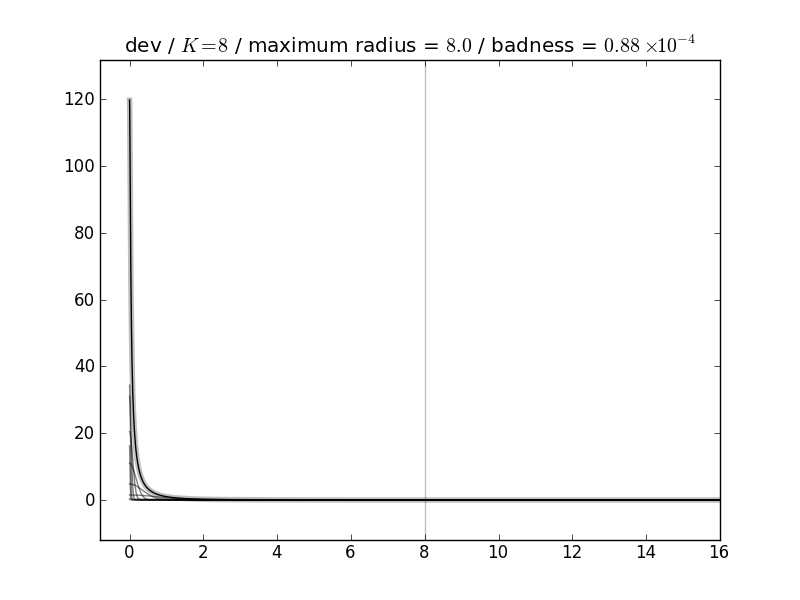
\includegraphics[width=\figwidth]{K08_MR08_LSD04_dev.png}
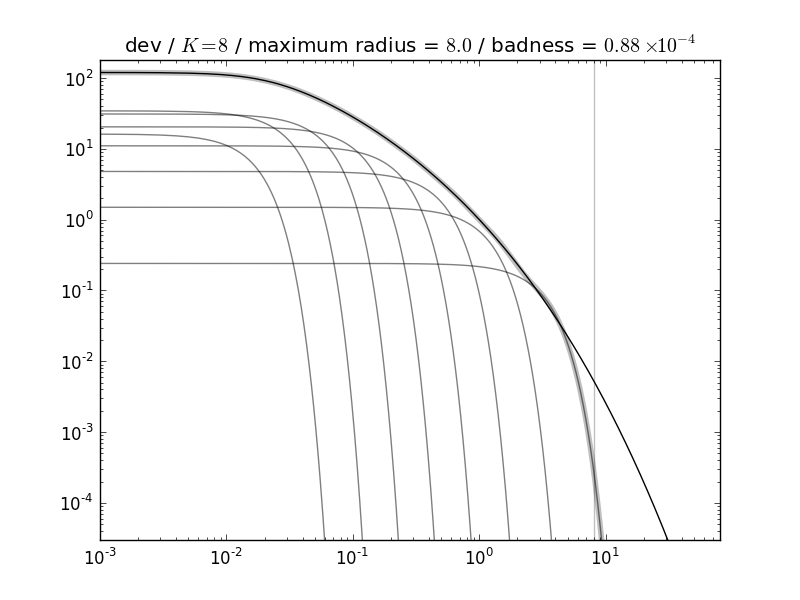
\includegraphics[width=\figwidth]{K08_MR08_LSD04_dev_log.png} \\
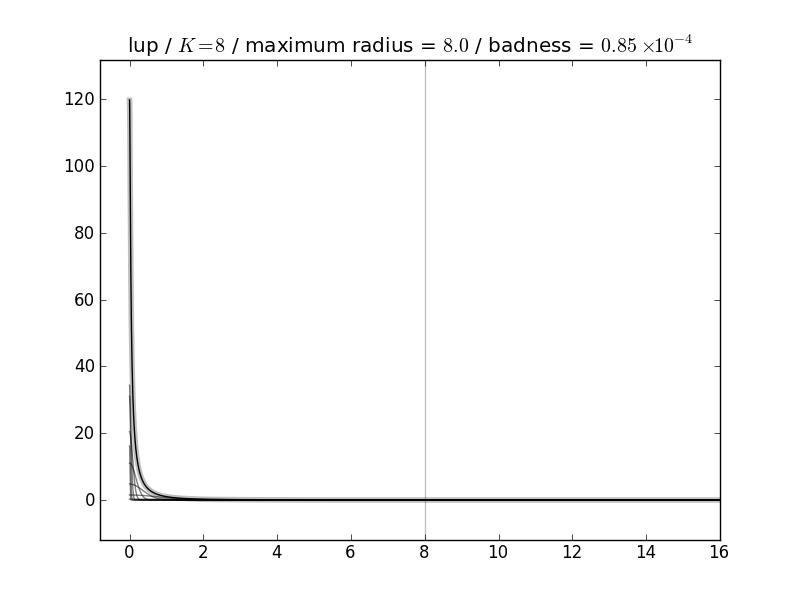
\includegraphics[width=\figwidth]{K08_MR08_LSD04_lup.png}
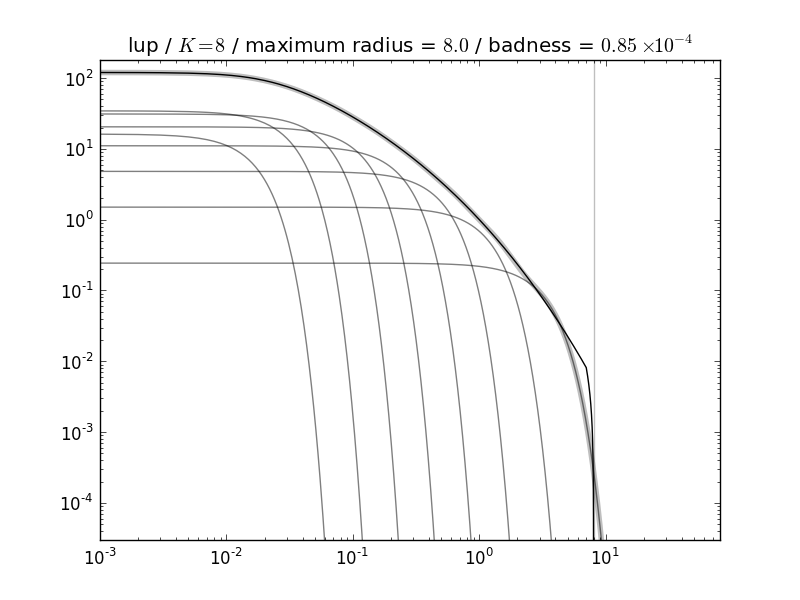
\includegraphics[width=\figwidth]{K08_MR08_LSD04_lup_log.png}
\end{figure}

\end{document}
